Referring to  Figure~\ref{fig:radii}, let $r$, $R$, and $r_9$ denote the radii of the incircle, circumcircle, and 9-point circle of a 3-periodic orbit, respectively. These are centered on $X_1$, $X_3$, and $X_5$, respectively \cite{coxeter67}. The Mittenpunkt $X_9$, is stationary at the elliptic billiard center over the 3-periodic orbit family \cite{reznik2019-intelligencer}.

\begin{figure}[H]
    \centering
    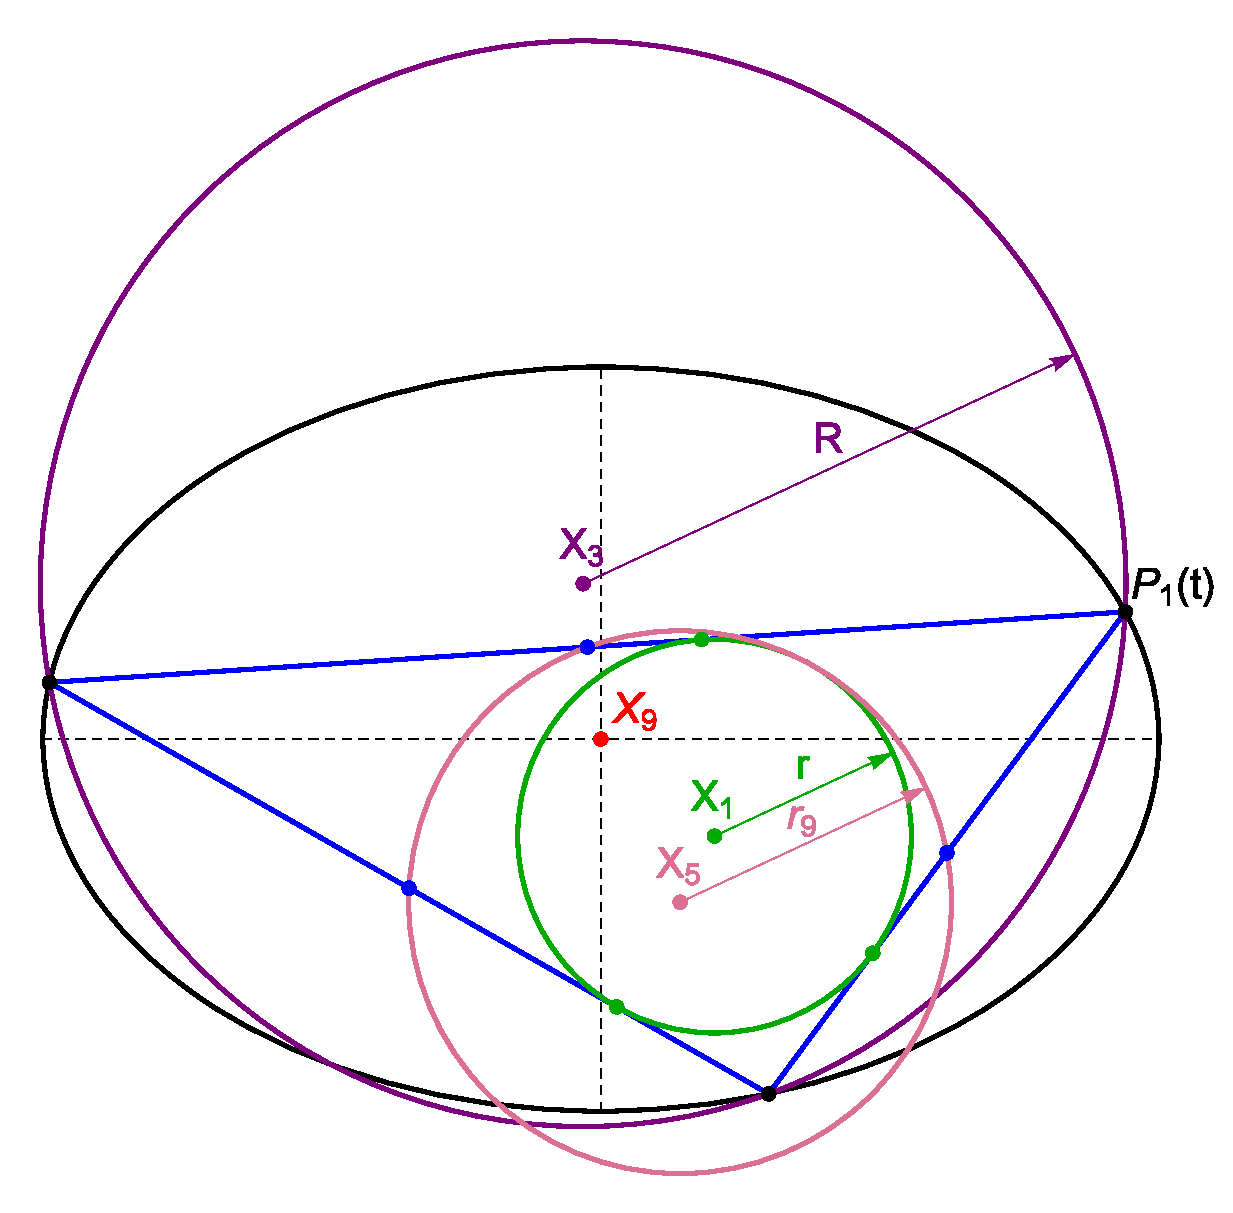
\includegraphics[width=.75\textwidth]{1040_Radii.eps}
    \caption{A 3-periodic orbit (blue), a starting vertex $P_1$, the incircle (green), circumcircle (purple), and 9-point circle (pink), whose centers are $X_1$, $X_3$, and $X_5$, and radii are the inradius $r$, circumradius $R$, and 9-point circle radius $r_9$. The Mittenpunkt $X_9$ is stationary at the billiard center \cite{reznik2019-intelligencer}.}
    \label{fig:radii}
\end{figure}

\noindent We now prove a result announced in  \cite{reznik2019-intelligencer}:

\begin{theorem}
\label{thm:rovR}
$r/R$ is invariant over the 3-periodic orbit family and given by
\begin{equation}
\label{eqn:rovR}
\frac{r}{R}=\frac{2 (\delta-b^2)(a^2-\delta)}{(a^2-b^2)^2}.
\end{equation}
\end{theorem}

\begin{proof}
Let $r$ and $R$ be the radius of the incircle and circumcircle, respectively. For any triangle \cite{coxeter67} we have

\begin{equation*}
 rR=\frac{s_1s_2s_3}{2 L}, 
\end{equation*}

\noindent where $L=s_1+s_2+s_3$ is the perimeter, constant for 3-periodic orbits; see equation \eqref{eqn:perimeter}. Therefore,

\begin{equation}
\frac{r}{R}=\frac{1}{2L} \frac{s_1s_2s_3}{R^2}\cdot
\label{eqn:rovR-cas}
\end{equation}

Next, with $P_1=(a,0)$, obtain a {\em candidate} expression for $r/R$. This yields \eqref{eqn:rovR} exactly. Using explicit expressions for orbit vertices (see Appendix~\ref{app:orbit-vertices}), derive an expression for the square of the right-hand side of \eqref{eqn:rovR-cas} as a function of $x_1$ and subtract from it the square of \eqref{eqn:rovR}. It can be shown $\left(s_1s_2s_3/R^2\right)^2$ is rational on $x_1$ \cite{reznik2020-loci}. For simplification, use $R=s_1 s_2 s_3/(4A)$, where $A$ is the triangle area. With a computer algebra system (CAS), show said difference is identically zero for all $x_1\in(-a,a)$.
\end{proof}

Though the ratio $r/R$ is invariant, the maxima and minima of $r$ and $R$ occur at the isosceles configurations of the 3-periodic orbits; see Figure~\ref{fig:rR-min-max}. 

\begin{figure}[H]
    \centering
    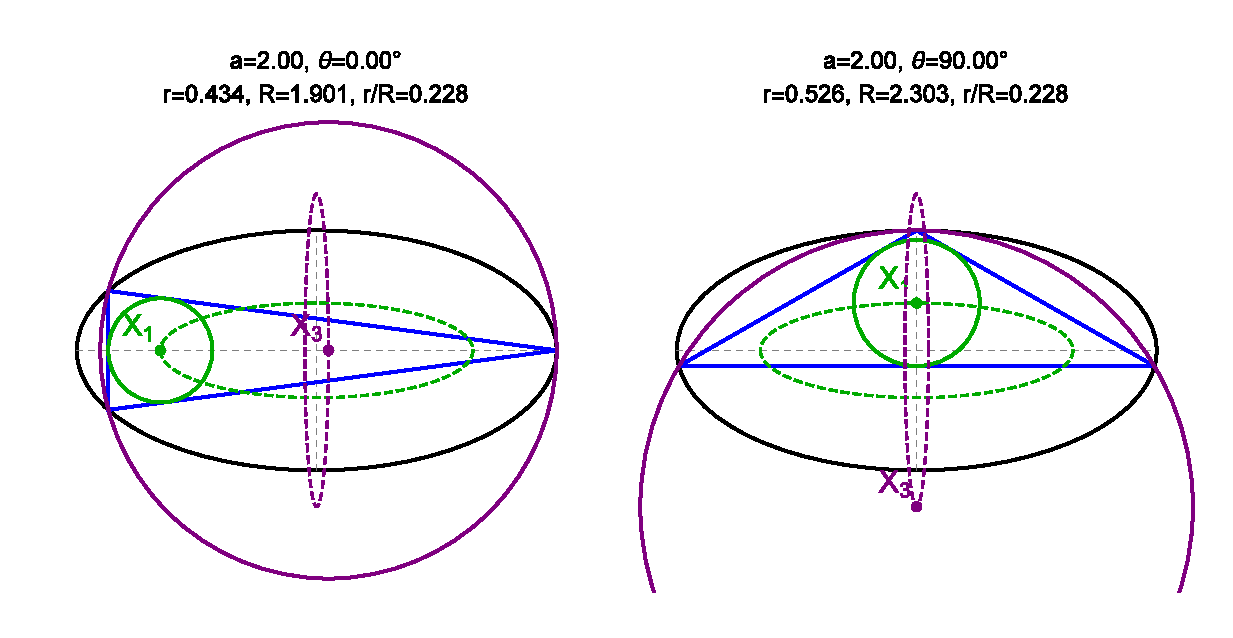
\includegraphics[trim={0 0.5cm 0 0},clip,width=\textwidth]{1060_radii_min_max_orbits}
    \caption{\textbf{Left}: When the 3-periodic orbit (blue) is a sideways isosceles triangle (one of its vertices   at either horizontal vertex of the elliptic billiard), $r$ and $R$ are minimal. The incircle and circumcircle are shown (green and purple, respectively), as are the loci of the incenter and circumcenter (dashed green and dashed purple, respectively). \textbf{Right}: When the orbit is an upright isosceles triangle (one vertex   the top or bottom vertex of the elliptic billiard), $r$ and $R$ are maximal.}
    \label{fig:rR-min-max}
\end{figure}

%\begin{proof}
%For any triangle we have the following relations.
%	\[rR= \frac{s_as_bs_c }{2(s_a +s_b +s_c	)}\]
%	\[R=\frac{r}{\cos A+\cos B+\cos C-1}=\sqrt{\frac{s_a^2+s_b^2+s_c^2}{8(1+  \cos A \cos B\cos C) }}\]
%\[ \frac{r}{R}= \cos A+\cos B+\cos C-1 \]
%\end{proof}

Note: The proof above and a few proofs below were obtained with the  assistence of   a Computer Algebra System. Indeed, expressions deriving from those in Appendix~\ref{app:orbit-vertices} quickly become unwieldy. We encourage the interested reader to produce simpler algebraic or, preferably, synthetic alternatives.

The three relations below hold for any triangle \cite{johnson29}. These will be used in subsequent corollaries.

\begin{eqnarray}
\sum_{i=1}^{3}{\cos\theta_i}&=&1+\frac{r}{R} \label{eqn:sum-cos} \\
\prod_{i=1}^{3}{|\cos\theta_i'|}&=&\frac{r}{4R} \label{eqn:exc-prod-cos} \\
\frac{A}{A'}&=&\frac{r}{2R}
\label{eqn:area-ratio}
\end{eqnarray}

\noindent where $\theta_i$ are the angles internal to the orbit, $\theta_i'$ are those of the excentral triangle (opposite to orbit $\theta_i$), and $A$ (respectively, $A'$) is the area of the orbit (respectively, excentral triangle); see Figure~\ref{fig:orbit-outer-inner}.

\begin{corollary}
The sum of the orbit cosines, the product of excentral cosines, and the ratio of excentral-to-orbit areas are all constant.
\end{corollary}

Note that the absolute value in \eqref{eqn:exc-prod-cos} can be dropped as the excentral triangle is always acute \cite{coxeter67}.

In \cite{reznik2019-intelligencer} we reported experiments that showed that the left-hand sides of \eqref{eqn:sum-cos} and \eqref{eqn:exc-prod-cos} were constant for all $N$-periodic orbits, whereas \eqref{eqn:area-ratio} was constant for odd $N$ only. These generalizations were subsequently proved \cite{akopyan2020-invariants,bialy2020-invariants}.

\begin{figure}[H]
    \centering
    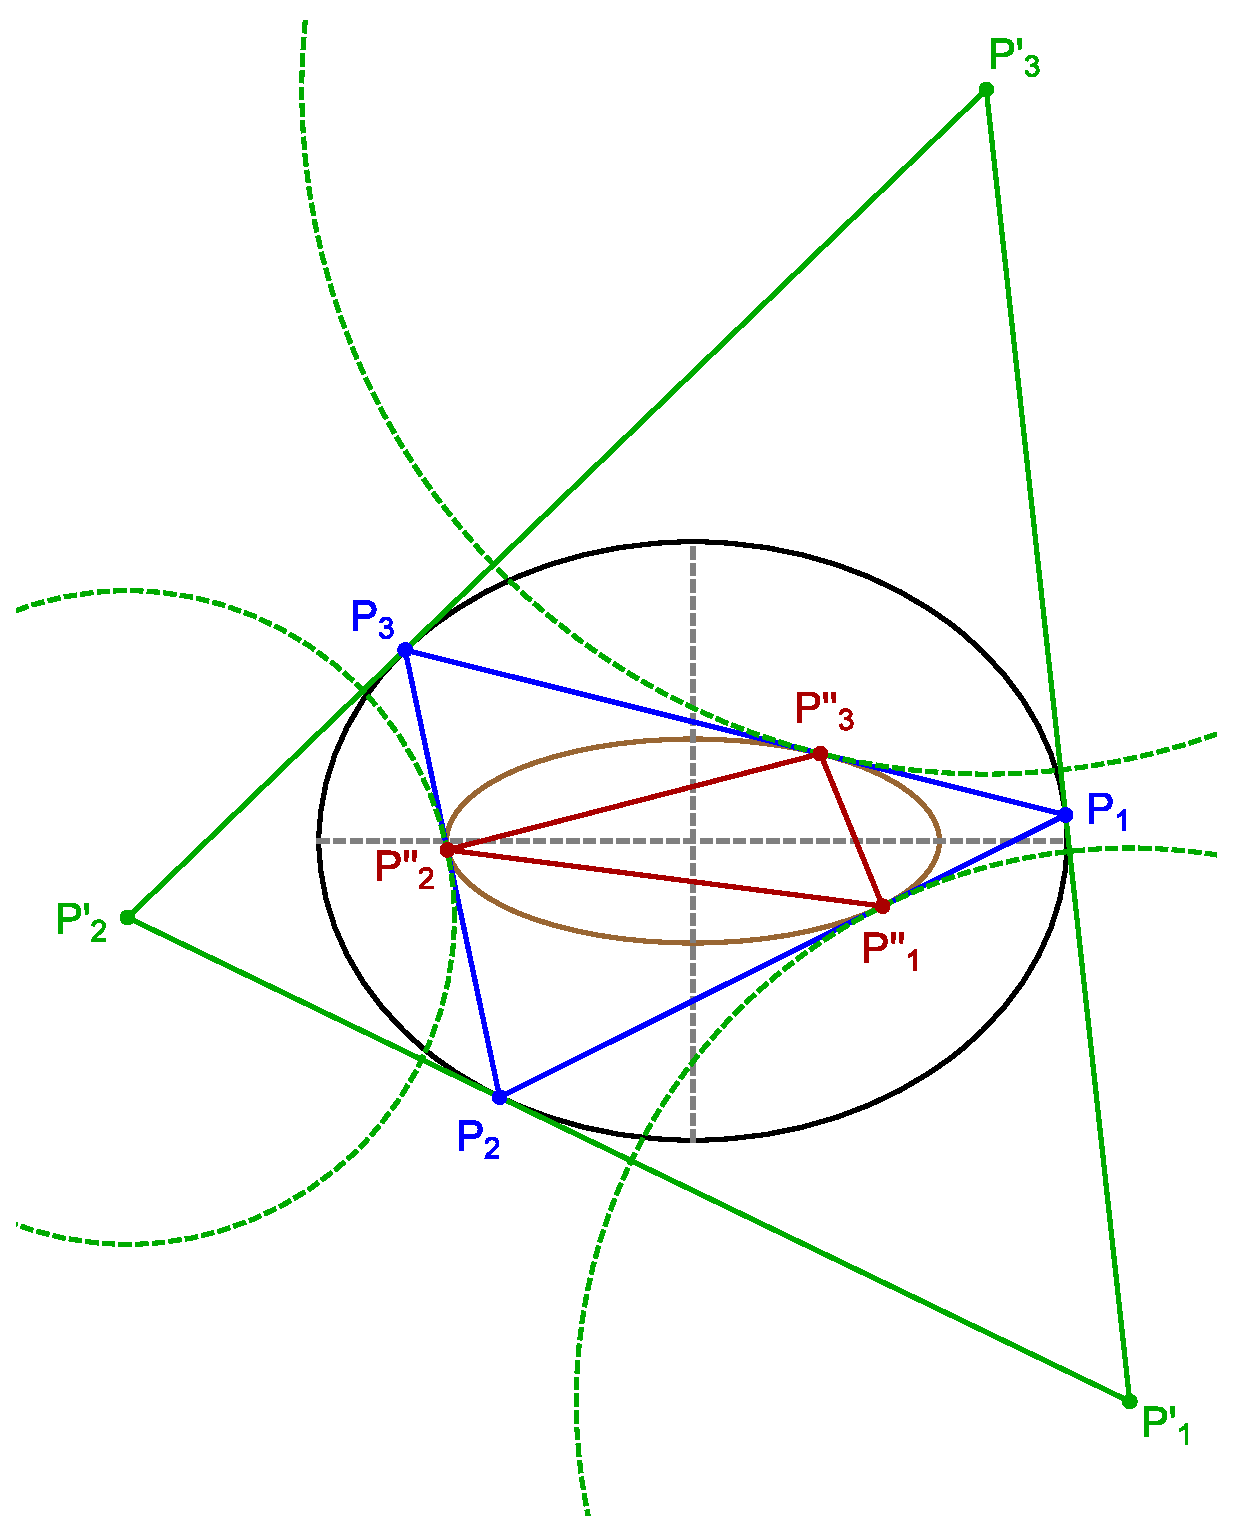
\includegraphics[width=.6\textwidth]{1090_orbit_outer_inner}
    \caption{An $a/b=1.25$ elliptic billiard is shown (black) as well as a 3-periodic orbit $T=P_1P_2P_3$ (blue). The orbit's excentral triangle $T'=P_1'P_2'P_3'$ (green) has vertices at the intersections of exterior bisectors (therefore it is tangent to the elliptic billiard at the orbit vertices). The extouch triangle $T''=P_1''P_2''P_3''$ (red) has vertices   where excircles (dashed green) touch each side. Said vertices are known to lie on the orbit's caustic (brown) as it is its Mandart inellipse \cite[Mandart Inellipse]{mw}.  $A,A',A''$ are the areas of $T,T',T''$, respectively \textbf{Video}: \cite[PL\#06]{reznik2020-playlist-proofs}}
    \label{fig:orbit-outer-inner}
\end{figure}

\subsection{Excentral-to-Extouch Area Ratio.}

Let $A''$ denote the area of the extouch triangle, whose vertices are where each excircle touches a side \cite[Extouch Triangle]{mw}; see Figure~\ref{fig:orbit-outer-inner}.

\begin{remark}  
The vertices of the orbit's extouch triangle lie on the caustic.
\end{remark}

Indeed, these are known lie on the Mandart inellipse, whose center is the Mittenpunkt $X_9$ \cite[Mandart Inellipse]{mw}; therefore it must be the caustic; see (\cite[PL\#06]{reznik2020-playlist-proofs}).

\begin{theorem}
$A'/A''$ is invariant and equal to $(2R/r)^2$.
\label{thm:area-ratio-outer-inner}
\end{theorem}

\begin{proof}
Combine the expressions for the area of the excentral \cite[Excentral Triangle]{mw} and extouch triangles \cite[Extouch Triangle]{mw} as a function of sidelengths $s_i$, inradius $r$, and perimeter $L$, obtain $A'/A=A/A''=(s_1 s_2 s_3)/(r^2 L)$. Since $A'/A=r/(2R)$  and $A'/A''=(A'/A)(A/A'')$, the result follows from direct calculations.
\end{proof}

\subsection{Billiard-to-Caustic Area Ratio.}

The $N=3$ caustic semi-axes are given by \cite{garcia2019-ellipses,reznik2020-loci}:

\begin{align}
a_c=&\frac{a\left(\delta-{b}^{2}\right)}{c^2},\;\;\;\;
b_c=\frac{b\left({a}^{2}-\delta\right)}{c^2}\cdot
\end{align}

Note that two concentric, axis-aligned ellipses produce a 3-periodic Poncelet family if and only if $a/a_c+b/b_c=1$ \cite{georgiev2012-poncelet}, which holds for the above $a_c,b_c$. 


\begin{corollary}
\label{cor:caustica_billiard}
Let $A_b$ and $A_c$ be the areas of the elliptic billiard and the $N=3$ confocal caustic, respectively. Then

\begin{equation}
\frac{A_c}{A_b}=\frac{r}{2R}\cdot
\label{eqn:caustic-area-ratio}
\end{equation}
\end{corollary}

\begin{proof}
As $A_c=\pi{a_c}{b_c}$ and $A_b={\pi}{a}{b}$, the result follows from equation~\eqref{eqn:rovR}.
\end{proof}

  Notice the caustic-to-billiard area ratio is equal to the orbit-to-excentral area ratio, equation~\eqref{eqn:area-ratio}. Recall also that the caustic semi-axes $a_c,b_c$ depend on $N$, i.e., equation  \eqref{eqn:caustic-area-ratio} is specific for the $N=3$ case.

The power of a point $Q$ with respect to a circle centered at $C_0$ of radius $\mu$ is given by $|Q-C_0|^2-\mu^2$ \cite[Circle Power]{mw}. Let $\mathcal{C}$ be the (moving) circumcircle to the 3-periodic orbits.

\begin{theorem}\label{thm:power_delta}
The power of the billiard center $O$ with respect to $\mathcal{C}$ is invariant and equal to $-\delta$.
\label{thm:delta-power}
\end{theorem}

\begin{proof}
 Consider an isosceles 3-periodic orbit with $P_1=[a,0]$,
 {\small  
 \[  \;  P_2   =\left[\frac {{a}^{2}\sqrt {2\,\delta-{a}^{2}-{b}^{2}}}{{a}^{2}-{b}^{2}},   
	\frac { \left(\delta  -{a}^{2}\right) b}{{a}^{2}-{b}^{2}}\right]\;\;
	 \text{ and  }\;\;  P_3= \left[{\frac {{a}^{2}\sqrt {2\,\delta-{a}^{2}-{b}^{2} }}{{a}^{2}-{b}^{2}}},
	{\frac { \left(  {a}^{2}-\delta \right) b}{{a}^{2}-{b}^{2}}}\right].
	\]
 }%
	Its circumcircle will be centered at $C_0=[ {\frac { {b}^{2}-\delta}{2b}},0]$ with circumradius $R_0=\frac {{b}^{2}+\delta}{2b}.$
	Therefore, the power of the center of the ellipse with respect to the circumcircle is given by  
	$$|OC_0|^2-R_0^2=\left(\frac { {b}^{2}-\delta}{2b}\right)^2 - \left(\frac {{b}^{2}+\delta}{2b}\right)^2=-\delta.$$

For a generic 3-periodic orbit, the stated invariance is confirmed via a CAS, using the explicit vertex expressions in \cite{garcia2019-ellipses} reproduced in Appendix \ref{app:orbit-vertices}.
\end{proof}



 
